% options:
% thesis=B bachelor's thesis
% thesis=M master's thesis
% czech thesis in Czech language
% english thesis in English language

\documentclass[thesis=M,english]{FITthesis}[2011/07/15]

% \usepackage[utf8]{inputenc} % LaTeX source encoded as UTF-8
% \usepackage[latin2]{inputenc} % LaTeX source encoded as ISO-8859-2
% \usepackage[cp1250]{inputenc} % LaTeX source encoded as Windows-1250

\usepackage{graphicx} %graphics files inclusion
\usepackage{algorithmic} %subfigures
% \usepackage{amsmath} %advanced maths
% \usepackage{amssymb} %additional math symbols

% % list of acronyms
% \usepackage[acronym,nonumberlist,toc,numberedsection=autolabel]{glossaries}
% \iflanguage{czech}{\renewcommand*{\acronymname}{Seznam pou{\v z}it{\' y}ch zkratek}}{}
% \makeglossaries

% \usepackage{listings}
% \usepackage{color}

% \definecolor{textbg}{RGB}{195,195,195}

% % % % % % % % % % % % % % % % % % % % % % % % % % % % % % 
% EDIT THIS
% % % % % % % % % % % % % % % % % % % % % % % % % % % % % % 

\department{Department of \ldots (SPECIFY)}
\title{Thesis title (SPECIFY)}
\author{Pavel Kachalouski} %author's name without academic degrees
\authorWithDegrees{Pavel Kachalouski \& degrees} %author's name with academic degrees
\supervisor{Your Supervisor's Name (SPECIFY)}
\acknowledgements{THANKS}
\abstractEN{Summarize the contents and contribution of your work in a few sentences in English language.}
\abstractCS{V n{\v e}kolika v{\v e}t{\' a}ch shr{\v n}te obsah a p{\v r}{\' i}nos t{\' e}to pr{\' a}ce v {\v c}esk{\' e}m jazyce.}
\placeForDeclarationOfAuthenticity{Olomouc}
\keywordsCS{Replace with comma-separated list of keywords in Czech.}
\keywordsEN{Replace with comma-separated list of keywords in English.}

\parskip 2mm

\begin{document}

% \newacronym{CVUT}{{\v C}VUT}{{\v C}esk{\' e} vysok{\' e} u{\v c}en{\' i} technick{\' e} v Praze}
% \newacronym{FIT}{FIT}{Fakulta informa{\v c}n{\' i}ch technologi{\' i}}

% \setsecnumdepth{part}
\chapter{Introduction}
\section{Motivation}
First major malicious internet-based attack was introduced in 1988 when one of the first Internet worms was released. Referred to as "The Morris Worm", it was written by Robert Tappan Morris and caused major interruptions across large parts of the Internet. Since 1988 Internet has greatly evolved and as a result increased number of internet-based attacks and network security became a really important issue. As an attempt to overcome this problem Intrusion Detection systems were developed. Such systems allow to monitor and possibly prevent attempts to intrude into or compromise the network resources.

In short it works as follows: you have a computer system. Your computer system is attached to the network and may be even to the Internet. You are willing to allow access from the network, by authorized people, but you are not however willing to allow unauthorized access to the system by anyone else. Typically, a firewall or authentication system is used to prevent unauthorised access. However, sometimes authentication systems and firewalling can be broken. Intrusion Detection is a set of mechanisms that are helps to detect unauthorised access to the system. Also Intrusion Detection systems may take some steps to deny access for intruders. Such systems are placed between firewall and system being secured and provide an extra layer of protection to that system.
\begin{figure}[h]
\centering
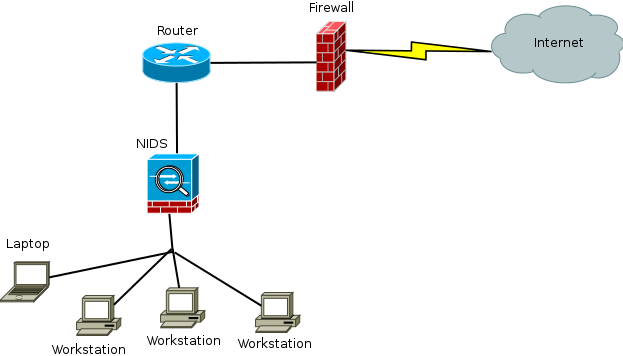
\includegraphics[scale=0.5]{images/Typical_NIDS.png}
\caption{Typical NIDS scenario.}
\end{figure}
Intrusion detection systems fall into two categories:
\begin{itemize}
\item Network based system. 
Such types of systems are placed in the network near the system that should be monitored. They monitor network traffic and examine whether it is withing acceptable boundaries.
\item Host based systems. 
Such types of detection systems are run on the system being monitored and determine if activity on the system is acceptable.
\end{itemize}
There are also more recent type of intrusion detection system which reside in the kernel of operation system and monitor on low-level system activity.

Most modern network intrusion detection and prevention systems use a set of rules that are compared to incoming and outcoming packets. Usually, a rule consists of a filter based on packet header information, a data that should be contained in the packet payload and an associated action that is taken in case filter and payload matching conditions are met.
Matching payload signatures is a resource-intensive process, accounting for about 75\% of the total CPU processing time of modern Network Intrusion Detection systems. The reason why is it so intensive is in the fact that most of the time, every byte of every network packet should be processed as a part of data searching algorithm that searches for matches along a large set of rules that apply for particular packet. As an example, most widely used open-source NIDS Snort has rule set with about 10000 strings. Searching every packet for all of this strings needs a lot of resources. With increasing number of internet-based attacks rules datasets grow every year creating additional load on NIDS systems. In the figure 1.2 is shown a general trend of the number of web-based attacks on web servers taken from Symantec Corporation report[TODO:add number].
\begin{figure}[h]
\centering
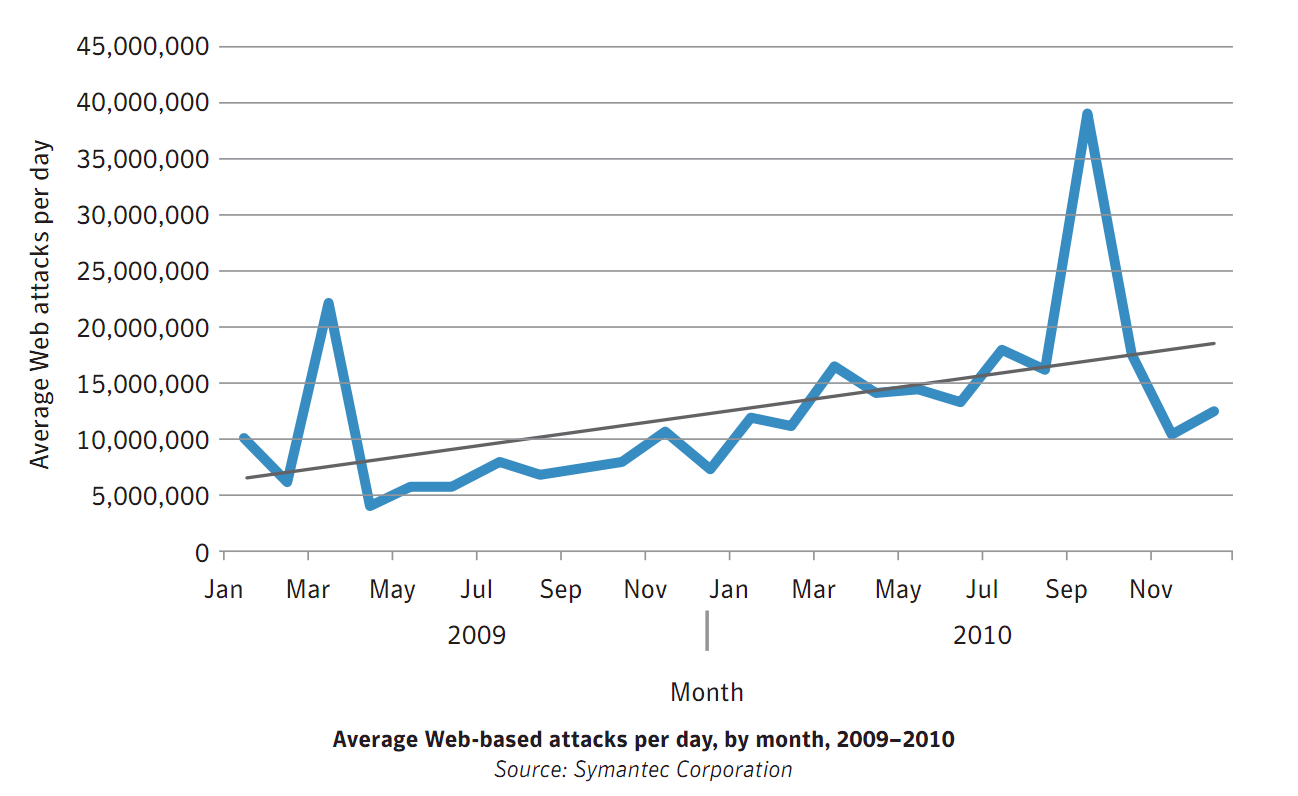
\includegraphics[scale=0.3]{images/web-attacks.png}
\caption{Average Web-based attacks per day, by month, 2009-2010. Source: Symantec Corporation.}
\end{figure}

The other source of high load on NIDS is constant grow of networks speeds. In the past 6 years, computer networks were characterized by a steady increase in the transfer rate, complexity and number of networked users. In 2009 the Internet traffic growth all over the world amounted to 40-50 \%, and according to Cisco company forecast [TODO:add number] global IP traffic will increase in the next 5 years, reaching by 2015 about 1 zettabyte of data transferred during one year.

Problem with high load on NIDS can be solved by using specialized network processing devices such as FPGA, ASIC, Network Processing Unit (NPU), or the TCP Offoading Engine (TOE). Nonetheless, the solutions may not be cost effective and easy to manage because they require special hardware and configurations.

\subsection*{Problem definition}
A quick packet processing in a NIDS over huge amount of data obtained from the network \textbf{is a must}. Perfomance of network data processing algorithms should be fast and should not interfere with the overall network perfomance (or interfere as little as possible).
The current factors related to the networks and traffic analysis systems listed below:
\begin{enumerate}
\item The number of network nodes and users are increasing. 
\item Network speed (bit rate) is gradually increasing.
\item The amount of network traffic is increasing heavily.
\item Analysis algorithms are getting more complex.
\item Databases of known threats grow resulting in high number of rules for matching.
\end{enumerate}

This thesis approach is to use heterogeneus computing, and more specifically use \textbf{graphic processing units} to perform network data analysis.

Heterogeneous computing is a way of computing some tasks using systems made up by different types of computational units. Computational unit types could be: a general-purpose processors (GPP), also known as central processor units (CPUs), which are usually the main processor of the most of the computing systems, and special-purpose processors (SPP). SPP are, for example, digital signal processors (DSP) or graphics processor units (GPU).

Graphics Processing Unit or GPU is essentially a dedicated hardware device that is responsible for translating data into a 2D image formed by pixels. GPU evolution is connected to the growing popularity and complexity of rendering programs like CAD (Computer Aided Design) programs and to 3D video games. These software required high computing capabilities which have to be satisfied by the GPUs. As a result engineers developed a highly parallel processor structure, which is able to execute many execution threads concurrently, and a high speed memory.

The interest to use GPUs to perform calculation tasks that are not suitable for GPUs began to grow in 2005. Developers and investigators were trying to use parallelism and memory bandwidth to enhance complex algorithms perfomance. GPUs are used for computations in molecular dynamics, quantum chemistry, bioinformatics, computational fluid dynamics, weather and climate forecasting and more other fields.

GPGPU (general-purpose computing on graphics processing units) at the beginning used GPUs as they were computing graphics tasks. Input data were encoded into image, then by using graphics libraries some operations were perfomed with an image and result data were decoded from image to its original form. Later companies realised that GPGPU could be an advantage for their business and invested in developing tools to make easier to use their products. NVIDIA developed CUDA (an acronym for Compute Unified Device Architecture) version 1.0 library in 2006, which enabled to run CUDA code written in special manner on some of their GPUs, while AMD developed ATI Stream technology that uses OpenCL language to write code executed on GPUs.

CUDA is the computing engine in Nvidia GPUs that is accessible to software developers through variants of industry standard programming languages. Programmers use 'C for CUDA' (C with Nvidia extensions and certain restrictions), compiled through a PathScale Open64 C compiler to code algorithms for execution on the GPU.
The main objective of this thesis is to develop open-source NIDS application which will inspect network traffic using classic CPU mode and heterogeneous CPU+GPU mode and compare perfomance of the two modes. 

In additional, the software should fulfill the following requirements:
\begin{itemize}
\item Open source. The application should be developed under the terms of open source software.
\item Application should be developed in C/C++ and C for CUDA languages.
\item Easy to use. Application should be easy to use for the users. NIDS rules should have easy format.
\item Application will analyze only TCP/IP traffic due to simplifications on the packet decomposition level.
\item Logging and offline analysis. Application should be able to store traffic for the future analysis in offline mode.
\end{itemize}

\section{Project overview}

\begin{figure}[h]
\centering
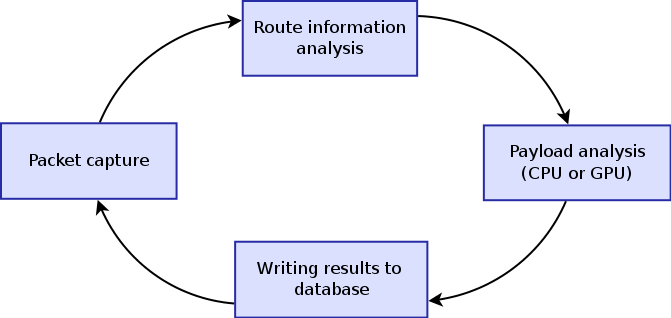
\includegraphics[scale=0.4]{images/workflow.png}
\caption{Application workflow.}
\end{figure}

The general application workflow is shown in the figure [TODO: add number].
The main stages of the workflow:
\begin{itemize}
\item \textbf{Packet capture}. Application captures traffic on one of the network interfaces for later analysis. Raw packet should be obtained from network for full analysis of route information on the next stage.
\item \textbf{Route information analysis}. Every packet is analyzed by means of type of the protocols used on network and transport layers and also destination and source IP address. If packet route information matches to any rule from the dataset it transported to the next stage of the workflow.
\item \textbf{Payload analysis}. Application looks for a string or regex in the packet payload.
\item \textbf{Writing result to a database}. On this stage all matched packets from the previous stage are written to a database with a message obtained from rule with which packet was matched.
\end{itemize}

\chapter{Background}
\section{Traffic analyzing: sniffers.}
Packet sniffer is a program or library which allows to intercept data packets transmitted over a certain network to which the system is connected throught a network card. Most popular known sniffing software is tcpdump[], Wireshark and OmniPeek. These programs are used for obtaining raw network packets and performing analyzing over obtained packets in order to represent them in a some visual form or dump to a file. There are also pure sniffing libraries, such as Libpcap (for UNIX like OS) and Winpcap (for Windows OS).

\subsection{How they work.}
The vast majority of network cards, support what is known as promiscuous mode or monitor mode. Normal operation of network cards when obtaining packets from the network (default configuration), compare the destination layer 2 (link layer) address to the one in use by the network card. If packet destination address and network card address in use match, or if the packet destination address is a broadcast address 1, packets are passed to the operating system, otherwise packets are dropped.

If promiscuous mode or monitor mode is enabled, network card passes all packets captured from the network to the operating system, even if they are not addressed to the system. Operating system later manages, using the packet filter engine, how to distribute packets to the applications. In the Unix-like systems, root privileges are required to enable promiscuous and monitor operation mode. Sniffer techniques rely on this functionality to do its job.

It is important to remark that capturing packets from a network is highly dependent of the type of the network used and of the topology and configuration of the network. Clear examples of this fact can be found in LAN (Local Area Network) networks based on the IEEE 802.XX (physical and link layer protocols) protocol macro-family, for instance in the IEEE 802.3 [9] protocol based networks, also known as Ethernet networks, and in the IEEE 802.11[10] based networks, so-called Wifi or Wireless networks. In the following subsections some details over sniffing on both network types are exposed.

\subsection{IEEE 802.3 sniffing details.}
In a typical IEEE 802.3 LAN network, a star topology is used, so all the nodes in the network are connected (through their own cable) to either a hub or a switch. 
Hubs are basically repeaters: packets coming from a certain port are retransmitted over the rest of the ports.
Switches instead, only send packets to the port where the destination host is connected, by previously identifying all the hosts connected to each port. Switched networks have better performance than not switched networks. Switches may perform other actions over traffic, such as filtering based on different protocol fields (link, network, transport and application protocol fields, depending on the switch), but this is beyond the scope of this thesis.
That means that if a switched network is used, only packets flowing to or from the particular host running the sniffer or broadcast packets will be captured. Several techniques have been used to overcome this problem:
\begin{itemize}
\item Using a hub: an obvious but bad solution is to use hubs instead of switches. It is not a valid solution as its performance is very reduced compared to switched networks and their production is practically discontinued.
\item Placing the sniffer in the gateway links as a bridge/router: this technique is widely used and has the advantage of being able to sniff packets from a lot of sub-networks by only placing one network tap. The disadvantage is that only traffic going through that link is captured, so internal traffic (between nodes in the same subnetwork or between different sub-networks) is not captured, which in some cases, like data centers for instance, is very relevant. In those cases the only solution is to use distributed sniffers, port mirroring or a combination of both of them. Figure 2.3 illustrates this technique with an example.
\item Switch port mirroring: some switches have what is called port mirroring or monitoring port 2 . If port mirroring is enabled, a copy of all the packets flowing in the switched are transmitted to the mirroring port selected. On networks formed by several switches, obtaining packets in a single host is more complex, and may require to use advanced switch capabilities like Cisco’s RSPAN or combine them with a distributed sniffer.
\item Distributed sniffer: distributed sniffers use a software based architecture to collect traffic in several network taps (hosts), and combine them to obtain them in a unique host. The main advantages of this type of systems are their scalability and flexibility. The drawbacks of this kind of systems are that distributed network sniffers have less performance than port mirroring due to overhead introduced by software architecture and the increase of network traffic. The figure 2.5 shows graphically the structure of a distributed sniffer platform.
\end{itemize}
\subsection{IEEE 802.11 sniffing details.}
IEEE 802.11 based networks share access medium, so it may be easier than IEEE 802.3 switched networks to capture packets, as having a network card being able to be set to promiscuous mode (actually monitor mode) is all the hardware required.
Nevertheless, some considerations have to be kept in mind. When placing a sniffer in a wireless network, some packets or even all the packets sent by a certain host may be lost, due to environment conditions (shadowing) and the physical position of the sniffer host and the other hosts in the network (attenuation due to propagation). IEEE 802.11 networks made up by several access points may increase capturing problems, due to the larger coverage area (and therefore the higher reception antenna gain needed when using a unique sniffer host).
Some approaches to solve these problems are:
\begin{itemize}
\item Capture packets in the wired network section: sometimes is preferable to sniff packets in the wired section rather than capturing them in the wireless subnetwork. This is conceptually similar to place a sniffer in the gateway link above mentioned, so the main disadvantage is that internal wireless traffic is not captured. This approach has also the drawback that link layer protocol (level 2) information is lost.
\item Distributed sniffer: usage of distributed systems. Pros and cons are similar than above mentioned.
\end{itemize}

\subsection{Libpcap.}
Libpcap is the capture library for Unix systems. Windows systems use a port of Libcap called Winpcap. This library offers the programmer an API to use BSD Packet Filter kernel facilities or any other Packet Filter kernel architecture that is based on Berkeley Packet Filter, to create user-level network capturing programs. Libpcap was released by the tcpdump developers in the Network Research Group at Lawrence Berkeley Laboratory. Libpcap offers the following capabilities: packet capturing from a network card, packet capturing from a file and capturing packets to save them into a file. Libpcap was extracted from the tcpdump program and made into a library. Development of Libpcap is in charge of tcpdump group [TODO: add number].

\subsection{Network traffic analysis techniques.}
In this section a brief introduction of main network traffic analysis techniques currently in use is exposed, focusing on the analysis procedures but also outlining some of the
analysis purposes which take advantage of them. But first, some considerations over the network traffic analysis inputs (network data) should be sketched out. The main input source of any network traffic analysis is the collection of packets captured from the network, commonly called the dataset or the analysis dataset. From that dataset which may contain all protocol header information as well as application an user information, a process of extracting (mining) the useful pieces of data for every particular analysis has to be carried out.
Datasets may also be broken up in smaller parts, resulting in data subsets, to later be analysed separately. The reasons of splitting dataset are usually performance issues with non-linear computing cost analysis algorithms, as working with large datasets may increase computing time exponentially, or to achieve a higher time resolution due to the reduced time interval of the datasubset. In these cases analysis are said to be performed over windowed datasets or simply called windowed analysis. Depending on the criteria followed to split the dataset into data subsets, two different types of windowed datasubsets can be obtained:
\begin{itemize}
\item Packet windowed datasubsets. Dataset is splitted in portions of equal number of packets each.
\item Time windowed datasubsets. Dataset is splitted in time intervals. The size of the subsets is unknown, and depends on the amount of traffic collected per second.
\end{itemize}

The usage and type of dataset windowing may affect to the results of the different analysis performed over it, and hence windowing parameters have to be taken into account when analysis results have to be evaluated and interpreted.

\subsection{Network traffic data inspection techniques.}
Network data inspection techniques obtain information of network data by inspecting network header fields of each packet, compute them and produce outputs or results.

\textbf{Packet decoding (packet analyzing)}
The simplest network data inspection possible is packet decoding, also called packet analysis, in which all header’s field are decoded and presented in a human readable way. Network analyzers like tcpdump, Wireshark or OmniPeek are some examples of packet decoding applications.
Packet decoding is used for the vast majority of purposes, being the most reliable security (intrusion detection, bandwidth abuse...) and network management and failure detection.
This kind of techniques are specially of interest in network security forensics analysis. Specific packet data extraction and analysis The extraction of pieces of data from the packets contained in the dataset instead of decoding all packet headers information, and processing them is a strategy used when particular aspects of traffic need to studied.
Different processing tasks can be performed over data collected:
\begin{itemize}
\item Graphical representation of raw data.
\item Statistical information and pattern extraction
\item Rule based (signature based) analysis, anomaly detection and policies.
\item Flow based analysis.
\end{itemize}
Graphical representation of raw data is of interest in many areas, principally in network monitoring, network management and security. Representations are usually in the form of 2D and 3D scatter plots, time based graphs, histograms, pie charts or diagrams. Network monitoring applications make an extensible usage of graphs like node state monitor graphs, throughputs and link performance graphs, source and destination hosts (IPs) histograms and scatter plots, service usage (TCP and UDP ports) histograms and scatter plots or routing diagrams. Some examples are shown in the figures below.

Statistical information and pattern extraction is a big field in network analysis. First and second order statistical moments, averages, time distributions and probability distributions functions are some of the basic statistical analysis that can be performed over network data. 
Obtaining interesting statistics over network traffic is widely used primarily in monitoring platforms. Average number of connections to a certain hosts, average inbound and outbound throughputs, transport and application layer protocol distribution, time distribution of connections to servers, time distribution of average network throughput are some examples. These statistics can also be applied for other purposes rather tan monitoring and network management, like security or marketing purposes (specially application level statics).

On the other hand, statistical pattern recognition or statistical pattern extraction is an extensive area related to network traffic analysis. They are applicable to security and
marketing fields. Due to the extension of this field and complexity, further information is given in the 2.2.2.2 section. Rule based (signature based) analysis and policies are all the analysis that inspect traffic searching packets that match a certain rule or signature. Rules or signatures are defined as values of certain headers fields or a combination of several values of certain headers fields. Rules may also define adequate field value intervals or thresholds. Rule based analysis is also frequently called signature pattern matching. There is quite a confusing usage of the term pattern over the network analysis literature, and particularly in network intrusion detection analysis literature: while some authors use the word pattern to designate statistical patterns (statistical user behaviour patterns, statistical usage patterns in general) like W.S. Chen in [31] or Yung Wang in [32], some others like Richard Bejtlich in several books like [33] use them to refer as rule based analysis. In this thesis be are going to refer to patterns as statistical patterns only. Rule based analysis techniques are used above all for security purposes and specially in signature based intrusion detection systems (NIDS), like Snort. Threshold rules are commonly used in security (for instance to detect DoS attacks and other resource abuse attacks) and also for network management purposes like for example in network link load monitoring.

In this sense, rules could be considered as policies, as certainly define the type and amount of traffic permitted and not permitted in the network. Flow based analysis techniques are focused in the treatment of network traffic as flows, as most information exchanged in a computer network is session or connection oriented and not packet oriented, so analysis can take advantage of it. A clear example of a typical network flow is a TCP connection, where data exchanged is ruled by the TCP state machine[26].
Their main applications are in the monitoring and security field. Regarding security, most NIDS like Snort, use flow based analysis techniques to detect possible threats, based on anomalies and well known attacks. Monitoring platforms on the other hand, inspect network traffic in search of flows, to generally list them or represent them in a diagram.

\textbf{Advanced statistical and signal processing techniques applied to the network traffic analysis.}
Since early 1990’s, researchers all over the world have devoted some of their efforts in the research of advanced statistical analysis techniques and also applying signal processing techniques to the network traffic analysis. The efforts have been centered in the network intrusion detection and prevention field, due to the fact that signature based NIDS (and NIPS) have important limitations detecting new security threats, as new rules for detection appear as new attacks and security threats are discovered. In addition,
signature based NIDS have the obvious drawback that rulesets have to be frequently updated. Platforms or applications that use statistical techniques for the network intrusion de-
tection are known as Statistical Network Intrusion Detection Systems or alternately Behaviour based Network Intrusion Detection Systems. This kind of NIDS rely on advanced statistical techniques, heuristic pattern extraction and signal processing to detect anomalies and classify network traffic.

Y. Wang exposes in his book [32] a general and up to date state-of-the-art of most reliable statistical techniques in the field of statistical network intrusion detection. There
is also an extensive set of publications from researchers over new statistical and signal processing techniques applied to network intrusion detection. Some of the techniques
are briefly introduced here.

\textbf{Linear and Nonlinear modeling methods.}
Significance tests, like χ2 (chi-square) test and t-test have been proposed for a simple network intrusion detection, examining frequency difference between two categorical variables and differences between two continuous variables respectively. Linear methods like logistic models, regression models, principal component analysis or clustered based analysis are some of the main methods suitable to use complex statistical modeling techniques to examine user behaviour based on network traffic data. 
Non linear methods are fundamentally based in AI (artificial intelligence) algorithms like Artificial neural networks, Fuzzy logic algorithms and K-nearest neighbour algorithms have also been found effective for aiding network intrusion detection decisions.

\textbf{Bayesian and probability approaches.}
Bayesian and probability approaches assume that parameters that are being studied are random rather than fixed parameters. Before looking at the current data, old information can be used to construct a prior distribution model for these parameters and therefore classify new data based on how likely various values of the unknown parameters are, and then make use of the current data to revise this starting assessment so that parameters can be considered random, not fixed. This attribute allows an intrusion detection systems to make a more precise decision based on the probability approach. Latent class model based analysis like proposed in Wang, Kim, Mbateng and Ho [34] or Bayes role based analysis like proposed by Barbard, Wu and Jajodia [35] are some examples of Bayesian and probability approaches.

\section{Intrusion detection.}
Intrusion detection is a process of detection undesired traffic on a network or device. An Intrusion Detection System is a combination of a physical device with a software which monitors network traffic in order to detect undesired activity and traffic that violates security policies. Different IDS tools are able also to store event information into log for later review or combine events with other information to make decisions about policies and losses. More functionalities provide IPS that can prevent or stop undesired traffic.

\textbf{Network-based Intrusion Detection (NID)}

A Network Intrusion Detection System (NIDS) is a type of IDS that monitors network traffic and analyzes packets deep on all levels of OSI model. Based on result of analyzis it makes decisions about the traffic type and suspicious activity. However, historically NIDS has been unable to operate in the following environment:
\begin{itemize}
\item Switched networks.
\item Encrypted networks.
\end{itemize}

\textbf{Host-based Intrusion Detection (HID)}

Host-based intrusion detection systems monitor and detect system and user activities on a given host. More complicated tools also offer policy management, data forensics statistical analysis and some access control. The difference between network-based intrusion detection and host-based intrusion detection is that NID deals with a traffic transmitted from one host to another while HID controls what is happening on the hosts themselfs.

Host-based intrusion detection is better fits to fight with internal threats, because it monitor and control specific user actions and file access. A lot of computer threats comes from the inside of organization, for example disgruntled employees or corporate spies.

\subsection*{Detection types}

\textbf{Signature-Based Detection}

Intrusion Detection may use signature-based detection to analyze traffic. Using such type of detection means that system is relying on known traffic data to analyze running traffic. An attacker can modify a little an attack to make it undetectable for such type of IDS. But regular expression-based rules give more power against such slightly changed attacks in the same time remaining very accurate.

\subsection*{Anomaly-Based Detection}
An IDS that looks at network traffic and detects data that is incorrect, not valid, or generally abnormal. This method is useful for detecting undesired traffic that is not specifically known. For instance, an anomaly-based IDS will detect that an Internet protocol (IP) packet is malformed. It does not detect that it is malformed in a specific way, but indicates that it is anomalous.

\subsection*{Stateful Protocol Inspection}
This type of detection is similar to anomaly-based detection, but it additionally inspects traffic on the transport layer and vendor-specific application layer, while anomaly-based detection is not doing it.

\section{Intrusion Detection Systems: A Brief History.}
The goal of intrusion detection is to monitor network assets to detect anomalous behavior and misuse. This concept has been around for nearly twenty years but only recently has it seen a dramatic rise in popularity and incorporation into the overall information security infrastructure. Beginning in 1980, with James Anderson's paper, Computer Security Threat Monitoring and Surveillance, the notion of intrusion detection was born. Since then, several pivotal events in IDS technology have advanced intrusion detection to its current state.

James Anderson's seminal paper, written for a government organization, introduced the notion that audit trails contained vital information that could be valuable in tracking misuse and understanding user behavior. With the release of this paper, the concept of "detecting" misuse and specific user events emerged. His insight into audit data and its importance led to tremendous improvements in the auditing subsystems of virtually every operating system. Anderson's conjecture also provided the foundation for future intrusion detection system design and development. His work was the start of host-based intrusion detection and IDS in general.

In 1983, SRI International, and specifically Dr. Dorothy Denning, began working on a government project that launched a new effort into intrusion detection development. Their goal was to analyze audit trails from government mainframe computers and create profiles of users based upon their activities. One year later, Dr. Denning helped to develop the first model for intrusion detection, the Intrusion Detection Expert System (IDES), which provided the foundation for the IDS technology development that was soon to follow.

In 1984, SRI also developed a means of tracking and analyzing audit data containing authentication information of users on ARPANET, the original Internet. Soon after, SRI completed a Navy SPAWAR contract with the realization of the first functional intrusion detection system, IDES. Using her research and development work at SRI, Dr. Denning published the decisive work, An Intrusion Detection Model, which revealed the necessary information for commercial intrusion detection system development. Her paper is the basis for most of the work in IDS that followed.

Meanwhile, there were other significant advances occurring at University of California Davis' Lawrence Livermore Laboratories. In 1988, the Haystack project at Lawrence Livermore Labs released another version of intrusion detection for the US Air Force. This project produced an IDS that analyzed audit data by comparing it with defined patterns. In a telephone interview with the author, Crosby Marks, a former Haystack Project team member and Haystack Labs employee said that, "searching through this large amount of data for one specific misuse was equivalent to looking for a needle in a haystack."

The subsequent iteration of this tool was called the Distributed Intrusion Detection System (DIDS). DIDS augmented the existing solution by tracking client machines as well as the servers it originally monitored. Finally in 1989, the developers from the Haystack project formed the commercial company, Haystack Labs, and released the last generation of the technology, Stalker. Crosby Marks says that "Stalker was a host-based, pattern matching system that included robust search capabilities to manually and automatically query the audit data." The Haystack advances, coupled with the work of SRI and Denning, greatly advanced the development of host-based intrusion detection technologies.

To kick off the '90s, UC Davis's Todd Heberlein introduced the idea of network intrusion detection. In 1990, Heberlein was the primary author and developer of Network Security Monitor (NSM), the first network intrusion detection system ( see Heberlein, L. et al. "A Network Security Monitor." Proceedings of the IEEE Computer Society Symposium, Research in Security and Privacy, May 1990, pp. 296-303.) NSM was deployed at major government installations where network traffic analysis provided massive amounts of information. This new awareness generated more interest in the field of intrusion detection and investments in that market increased significantly. Heberlein's contributions also extended to the DIDS project where, along with the Haystack team, he introduced the first idea of hybrid intrusion detection. The work of the Haystack project and the introduction of the Network Security Monitor revolutionized the IDS field and brought it into the commercial world.

Commercial development of intrusion detection technologies began in the early 1990s. Haystack Labs was the first commercial vendor of IDS tools, with its Stalker line of host-based products. SAIC was also developing a form of host-based intrusion detection, called Computer Misuse Detection System (CMDS). Simultaneously, the Air Force's Cryptologic Support Center developed the Automated Security Measurement System (ASIM) to monitor network traffic on the US Air Force's network. ASIM made considerable progress in overcoming scalability and portability issues that previously plagued NID products. Additionally, ASIM was the first solution to incorporate both a hardware and software solution to network intrusion detection. ASIM is still currently in use and managed by the Air Force's Computer Emergency Response Team (AFCERT) at locations all over the world. As often happened, the development group on the ASIM project formed a commercial company in 1994, the Wheel Group. Their product, NetRanger, was the first commercially viable network intrusion detection device. Nonetheless, commercial intrusion detection systems developed slowly during these years and only truly blossomed towards the latter half of the decade.
The intrusion detection market began to gain in popularity and truly generate revenues around 1997. In that year, the security market leader, ISS, developed a network intrusion detection system called RealSecure. A year later, Cisco recognized the importance of network intrusion detection and purchased the Wheel Group, attaining a security solution they could provide to their customers. Similarly, the first visible host-based intrusion detection company, Centrax Corporation, emerged as a result of a merger of the development staff from Haystack Labs and the departure of the CMDS team from SAIC. From there, the commercial IDS world expanded its market-base and a roller coaster ride of start-up companies, mergers, and acquisitions ensued. (The next section, Players, discusses these developments.)

Currently, market statistics show that IDS is amidst the top selling security vendor technologies and should continue to rise. Furthermore, government initiatives, such as the Federal Intrusion Detection Network, (FIDNet) created under Presidential Decision Directive 63, are also adding impetus to the evolution of IDS. Advancements in IDS will ultimately push security technology into a whole new arena of automated security intelligence.

\section{GPUs}
Graphical processor units commonly referred to them as GPUs and occasionally called visual processing units or VPUs, are a specialized type of processors that its purpose is to offload 3D graphics rendering from the microprocessor or CPU. The history of GPUs started in 1970s, where ANTIC and CTIA chips provided for hardware control of mixed graphics and text mode on Atari 8-bit computers. The ANTIC chip was a special purpose processor, that mapped text and graphics data to the video output.

Later, in 1984 the IBM Professional Graphics Controller appeared as one of the first 2D/3D graphics accelerators available for the IBM PC architecture compatible systems. IBM’s chip did not succeed, due to the lack of compatibility with already existing programs and due to its high price. The first mass-market computer to include a dedicated graphics processor was the Commodore Amiga, that was launched in 1985. The dedicated graphics processor from Amiga was the first full graphics accelerator as offloaded practically all video operations from the CPU.

By the time, IBM’s 8514 graphics system was the first PC video cards to implement 2D primitives in hardware. In 1991, S3 manufacturer introduced the S3 86C911 to the market, which claimed to be the first single-chip graphics card to implement 2D acceleration functions in hardware. The rest of the manufacturers followed the 86C911 model, and by 1995, all major PC graphics processor vendors had added 2D hardware acceleration support to their chips. During the first half of 1990s decade, CPU based real-time 3D graphics were becoming increasingly significant, specially in the CAD (Computer Aided Design) field and specially in computer video games. As video games gained popularity, and the consequent increasing demand of 3D hardware acceleration, graphics manufacturers started the development of 2D and 3D graphics accelerators. This milestone was reached with the launch of Verite V1000 chip in 1996 by Rendition.

During the second half of 1990s decade, and thanks to the increasingly success of 3D graphic programs, fundamentally video games, several manufacturers appeared to compete over the GPU market. By the end of 1990s, manufacturers leaders were 3dfx, ATI and NVIDIA. NVIDIA launched the Geforce 256 in 1999 being the first card on the market with hardware transform and lighting capabilities, adopting new hardware solutions that set the precedence for future designs like pixel shaders and vertex shaders. 

During the early 2000s, thanks to the OpenGL API, a multiplatform and multilanguage API that was created in 1992 by Silicon Graphics Inc. to help programmers draw 3D images, and new the hardware architectures that allowed each image pixel be processed by a short program that could include additional image textures as inputs and geometric vertex be processed similarly, 3D applications experienced a major graphical capability improvement.The first device that supported vertex shaders programming was the NVIDIA’s Geforce 3. In 2000 3dfx was acquired by NVIDIA. From that point to the present, the market of high performance GPU chips has been dominated by NVIDIA on one hand, with an estimated market-share of 63.46\% in October of 2009 according to [38], and ATI, with and estimated of 28.97\% of market-share according to [38] at the same date. 

The latest chips of NVIDIA are the G80 and G90 chip family (Geforce 8 and 9 ) generation. Recently NVIDIA has published a new architecture for the CUDA enabled chips with the code name Fermi[39], which will have 512 cores integrated in the chip, as well as bigger L1 and L2 cache memory sizes and memory error correction among others, making it more suitable for general purpose computing. For his part ATI has developed Radeon 5000 family, with the Evergreen graphic chipsets.

\subsection{GPGPU: general-purpose computing on graphics processing units.}
GPGPU stands for General-Purpose Computing on Graphics Processing Units. Since 2003, several researchers like Harris, Mark J., William V. among others [40], outlined that current architecture of high performance GPUs in terms of FLOPS (FLoating-point Operations Per Second), with programmable fragment and vertex shaders that enabled the programmers to create more realistic and complex graphics, could be used for other purposes rather than graphic calculations.

The motivation of GPGPU was performance improving of computing algorithms, and particularly to overcome limitations of traditionally CPU based computing: the instruction-level parallelism wall and the memory wall. On one hand, although GPUs architecture offer a limited set of operations to be performed over data, they have the ability to process many of them in parallel, thanks fundamentally to the programmable shaders that were added to the GPU processor’s pipelines. GPUs are able to compute many vertices or fragments of graphics in the same way in so-called streams. A stream is simply a set of elements that require similar computation, providing data parallelism, and kernels are the functions that are applied to each element in the stream.

In the other hand, the usage of graphical processor units have another important advantage over traditionally computing CPU based model; its memory bandwidth. In the last decade the gap between CPU and memory speed have kept growing, and thus memory latency has become a major bottleneck in CPU computing, specially in applications with an intensive usage of memory. The evolution of theoretical single precision floating point operations (FLOPS) [2] for both Intel based CPU processors and NVIDIA based GPU processors is shown in the figure 2.10. 

First attempts of using GPUs with other purposes rather than graphics, required to transform or convert complex algorithms and data into a graphics, to be able to use the GPU through graphics libraries (like OpenGL) to solve them and later revert the transformation. 

NVIDIA, conscious that GPGPU could be an important boost for the GPU market and also knowing that the current approaches for using GPUs for general purpose programming required a high level of knowledge and was a tedious job, started developing an SDK with the purpose of simplifying the task of GPGPU programming. The result of this development was CUDATM (Compute Unified Device Architecture), that was launched in November 2006. 

CUDA is a parallel computing architecture that enables programmers to use both CPU and GPU processors to cooperate in a single program, using a computing paradigm known as heterogeneous computing. Software developers are able to program general purpose functions or routines to be run on the GPU by simply use “C for CUDA” (C with NVIDIA extensions) while the rest of the program is still executed in the CPU. 

CUDA has become widely used in many areas such as physics simulations, scientific and medical simulations, signal processing, cryptography or audio and video processing among others. ATI also launched his own GPGPU SDK called Stream SDK, but at the time Stream SDK has not been as successful as CUDA.

\subsection{CUDA architecture and programming model for GPGPU.}

The CUDA SDK allows programmers to code parts or functions of a general purpose program to be executed in the GPU using C language with some extensions. The main three key abstractions that are exposed to the programmer as the C extensions are: a hierarchy of thread groups, shared memories and thread barrier synchronization. CUDA programmers have to partition the algorithms or parts of the code that are going to be boosted using the GPU into coarse sub-problems that can be solved independently in parallel, and then into smaller pieces that can be solved cooperatively in parallel. Functions executed into the GPU are called kernels, the rest of the code, and particularly
high control intensive parts of the code, are executed on the CPU. 

Kernels are functions designated with global attribute. When they are called, kernels throw a total number of N threads. To achieve a good performance in general, kernels should throw thousands of threads. Figure 2.11 show kernel’s thread organization of model. The N threads thrown by the kernel are organized in 2D array of blocks called grid 3 , each of this blocks containing a 3D array of threads. The number of threads, and their organization cannot be modified during the kernel execution. The programmer may use or not multidimensional block and grid organization according to their needs, simply not using (0 value) the dimensions not needed. 

The programmer can access to the current thread block ID dimensions values with variables blockIdx.x and blockIdx.y respectively. Likewise, the programmer can access to current thread ID dimension with variables threadIdx.x, threadIdx.y and threadIdx.z respectively. The combination of blockIdx and threadIdx complex variables values identify unequivocally each thread, and are used to perform ordered data accesses and execute code conditionally depending on the thread and block IDs. Currently, CUDA based programs have the restriction of a maximum of 65536 (216) threads and the limitation of 512 threads/blocks per dimension due to current GPU architectures (Tesla architecture).

The code contained in the figure 2.12 shows a simplified example of a kernel call, throwing vecAdd kernel with a 1D grid organization and 1D thread block organization, throwing NB blocks, with NT threads per block. Some coding details, like memory data transfers from CPU to host are omitted for simplicity.


\setsecnumdepth{all}
\chapter{Analysis and design}

\section{Developing tools and methodology.}
The tools and programming languages selected for implementing application are:

Languages:

\begin{itemize}
\item \textbf{C++}: due to perfomance requirements and supporting of object oriented features (classes, inheritance), C++ is used for developing the whole program, instead of the CUDA device code part, where C dialect for CUDA is used.
\item \textbf{CUDA}: CUDA uses C language with additional features to perform general purpose calculations in the GPUs.
\end{itemize}

Libraries:

\begin{itemize}
\item \textbf{Libpcap}: is packet-capture library for retrieving packets from the Packet Filter.
\item \textbf{QT}: is a cross-platform application framework for developing application with a rich graphical interface. It is used for building GUI part of the application.
\item \textbf{Boost}: is a set of libraries that extend the functionality of the C++ programming language. From boost libraries components for processes synchronization were used (semaphores and mutexes). Also boost.spirit parser is used to parse rules dataset.
\item \textbf{Sqlite}: is a software library that implements a SQL database engine and is used to store results.
\end{itemize}

The methodology used has been the spiral model.
\begin{figure}[h]
\centering
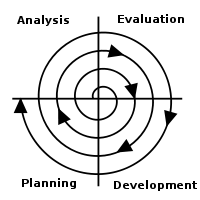
\includegraphics[scale=0.7]{images/spiral-model.png}
\caption{Spiral methodology used in the developing process of the application.}
\end{figure}

In this methodology, the process of determining requirements, analyzing possible risks, implementing, testing and planning (results evaluation), are performed during the whole project. The number of rotating through the spiral depend on the found implementation issues, the precision of objective definition in the early stages of the development and the requirements accomplishment of the current implementation.

\section{NIDS rules.}
NIDS rules dataset has a simple text format. Each line of the text file contain rule in the following format:


\begin{figure}[h]
\centering
\begin{verbatim}
action protocol src_ip src_port direction dst_ip dst_port {options}
\end{verbatim}
\caption{Rule format.}
\label{fig:rule_format}
\end{figure}

\textbf{Action} could be an \textbf{alert} or \textbf{log}, where 'alert' means that if case rule is matched against some packet it should be alerted to user, for example highlighted with a red color in a GUI. If rule starts with a 'log' action it means that packet matched against rule will be logged into a database without any specific actions for gaining user attention.

\textbf{Protocol} is a packet's protocol type. Because of simplifications only 'tcp' is supported by developing application.

\textbf{Src\_ip} is a source IP address of the packet. IP address is written in a standard form '192.168.0.1' where each position could be a range, for example '192.168.0-20.1'. Also instead of any position in the IP address, '*' symbol could be used to accept all values on that position. For example '192.168.*.*'.

\textbf{Src\_port} is a source TCP port. It is a value from 0 to 65535, or range, for example 5-1234, or '*' symbol which means any port.

\textbf{Direction} is a string "\textendash\textgreater". At this moment only this direction string is supported.

\textbf{Dst\_ip} is a destination IP address written in the same format as source IP address.

\textbf{Dst\_port} is a destination TCP port written in the same format as a source TCP port.

\textbf{Options} are parameters that specifies payload analysis. Within options should be a \textbf{content} or \textbf{pcre}. Content specifies a string which is searched within a packet payload. Also content string could contain raw bytes which should be written within '\textbar' symbols. Example of the content option with a string and raw bytes \textbf{content:"searchedstring\textbar00 01 02\textbar"}.\newline Pcre specifies the searched string as a regular expression. Example of pcre option \textbf{pcre:"\textasciicircum(some)*regex"}. The reason of dividing searched string on content and pcre is that all content strings are compiled into one DFA while each pcre is compiled in its own DFA and could consume much more memory. Options may contain parameters \textbf{offset} and \textbf{length} which means position in a payload from which searching should be started and number of bytes from the start position to observe. And finally \textbf{msg} parameter could be withing options. It is a simple string that should be logged or alerted to user when some packet matches against the rule.

\section{Application design overview.}
The main objective of this thesis is to design and implement simple NIDS application capable to analyze network traffic using GPUs, specifically using CUDA. 
\subsection*{Pattern matching.}
Pattern matching is the most heavy operation that affects the NIDS perfomance. Pattern matching algorithms can be classified into single-pattern and multi-pattern algorithms.

Single-pattern algorithms work in a way that each pattern is searched in a given text individually. Therefore for k searched patterns algorithm should be repeated k times. Some of the widely used algorithms are Knuth-Morris-Pratt and Boyer-Moore. Knuth-Morris-Pratt is able to skip characters when a mismatch occurs in the comparison phase using a partial match table for each pattern. Each table is built by preprocessing every pattern separately. Boyer-Moore is the most widely used single-pattern algorithm. Its execution time can be sublinear if the suffix of the string to be searched for appears infrequently in the input stream, due to the skipping heuristics that it uses.

Multi-pattern matching algorithms search a set of patterns in a text simultaneously. It is done by preprocessing all patterns that could be searched into an automation which is used during searching phase. The automation may be represented as a trie, a table or combination of the two. Such algorithms searches each byte from the text only once. Also such algorithms scales much better that single-pattern. Example of multi-pattern algorithms: Aho-Corasick, Wu-Manber and Commentz-Walter.

Previous section introduced NIDS rule which could contain \textbf{content} or \textbf{pcre} patterns that should be searched withing payload. As there could be a lot of rules and a lot of contents it was decided to use Aho-Corasick algorithm to search all content string simultaneously within packet payload. 

The algorithm consists of two parts. In the first part we construct from the set of patterns a finiste state machine; in the second part we apply the packet payload as input to the pattern matching machine. The machine signals whenever it has found a match for a keyword. The pattern matching machine consists of a set of states. Each state is represented by a number. The machine processes the text by successively reading symbols from input string, making state transitions and occasionally emitting output. The behaviour of the pattern matching machine is dictated by three functions: a goto function \emph{g}, a failure function \emph{f} and an output function \emph{output}. Figures \ref{fig:goto_function}, \ref{fig:failure_function} and \ref{fig:output_function} shows the functions used by a pattern matching machine for a set of keywords (he, she, his, hers).

\begin{figure}[h]
\centering
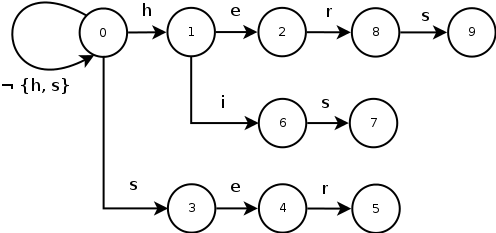
\includegraphics[scale=0.5]{images/goto_function.png}
\caption{Aho-Corasick goto function.}
\label{fig:goto_function}
\end{figure}

\begin{figure}[h]
\centering
\begin{tabular}{l l l l l l l l l l}
\emph{i}       & 1 & 2 & 3 & 4 & 5 & 6 & 7 & 8 & 9 \\
\emph{f(i)}    & 0 & 0 & 0 & 1 & 2 & 0 & 3 & 0 & 3 \\
\end{tabular}
\caption{Aho-Corasick failure function.}
\label{fig:failure_function}
\end{figure}

\begin{figure}[h]
\centering
\begin{tabular}{l l}
\emph{i} & \emph{output(i)} \\
2 & {he} \\
5 & {she, he} \\
7 & {his} \\
9 & {hers} \\
\end{tabular}
\caption{Aho-Corasick output function.}
\label{fig:output_function}
\end{figure}

One state (usually 0) is designated as a start state. In figure \ref{fig:goto_function} the states are 0, 1,...,9. The goto function \emph{g} maps a pair consisting of state and an input symbol into a state or the message fail. The directed graph in figure \ref{fig:goto_function} represents the goto function. The absence of an arrow indicates \emph{fail}. Thus, g(1, \emph{s}) = \emph{fail} for all input symbols \emph{s} that are not 'e' or 'i'.

The failure function \emph{f} maps a state into a state. The failure function is consulted whenever the goto function reports \emph{fail}. Certain states are designated as output states which indicate that a set of keywords has been found.

An operating cycle of a pattern matching machine is defined as follows. Let s be the current state of the machine and a the current symbol of the input string x.
\begin{enumerate}
\item If \emph{g(s, a) = s'}, the machine makes a goto transition. It enters state s' and the next symbol of x becomes the current input symbol.
In addition, if  \emph{output(s')  empty}, then the machine emits the set \emph{output(s')} along with the position of the current input symbol. The operating cycle is now complete.
\item If \emph{g(s, a) = fail}, the machine consults the failure function \emph{f} and is said to make a \emph{failure} transition. If \emph{f(s)=s'} the machine repeats the cycle with s' as the current state and a as the current input symbol.
\end{enumerate}
Initially, the current state of the machine is the start and the first symbol of the text string is the current input symbol. 

\begin{figure}
\textbf{Input.} A text string $x = a_1 a_2 ... a_n$ where each $a_i$ is an input symbol and a pattern matching machine M with goto function \emph{g}, failure function \emph{f}, and output function \emph{output}.\\
\textbf{Output.} Locations at which keywords occur in x.\\
\textbf{Method.}
\begin{algorithmic}
\STATE $state \leftarrow 0$
\FOR{$i=1$ to $n$}
\WHILE{$g(state, a_i) = fail$}
\STATE $state \leftarrow f(state)$
\ENDWHILE
\STATE $state \leftarrow g(state, a_i)$
\IF{$output(state) \neq empty$}
\PRINT i
\PRINT $output(state)$
\ENDIF
\ENDFOR
\end{algorithmic}
\caption{Aho-Corasick pattern matching machine algorithm.}
\label{fig:ac_search_pseudocode}
\end{figure}

\begin{figure}
\textbf{Input.} Set of keywords K={$y_1$, $y_2$,..., $y_k$} \\
\textbf{Output.} Goto function \emph{g} and a partially computed output function \emph{output}.\\
\textbf{Method.}
\begin{algorithmic}
\STATE $state \leftarrow 0$
\FOR{$i=1$ to $n$}
\WHILE{$g(state, a_i) = fail$}
\STATE $state \leftarrow f(state)$
\ENDWHILE
\STATE $state \leftarrow g(state, a_i)$
\IF{$output(state) \neq empty$}
\PRINT i
\PRINT $output(state)$
\ENDIF
\ENDFOR
\end{algorithmic}
\caption{Aho-Corasick pattern matching machine algorithm.}
\label{fig:ac_search_pseudocode}
\end{figure}

Figure \ref{fig:ac_search_pseudocode} shows Aho-Corasick matching machine algorithm pseudocode. Pseudocodes for construction of \textbf{Goto}, \textbf{Failure}, and \textbf{Output} are shown in figures \ref{fig:ac_goto_pseudocode}, \ref{fig:ac_fail_pseudocode}, \ref{fig:ac_output_pseudocode}.


\subsection*{Packet filtering based in route information.}


Application design is divided in several components. The diagram contained in figure \ref{fig:app_architecture} show the relationship between components.

\begin{figure}
\centering
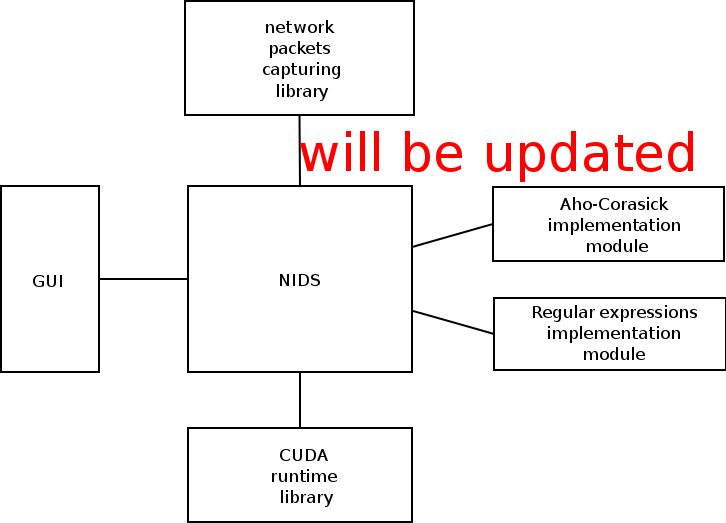
\includegraphics[scale=0.5]{images/app_architecture.png}
\caption{Relation between application components.}
\label{fig:app_architecture}
\end{figure}

\begin{itemize}
\item \textbf{GUI}. Component which implements user interactions with a program. Application has simple window-based interface which allows to perform all major manipulations with the application like starting capturing traffic, stop capturing, switching analyzing mode, saving traffic into the file, etc.
\item \textbf{Network packets capturing library}. Application itself doesn't capture packet from the kernel, because it is not a trivial task. Instead, program uses external library for packet capturing.
\item \textbf{NIDS}. The main component of the system. Uses all others modules to read rules, start capturing and analysing of packets. Stores results of analyzing into a database and updates counters which are used within NIDS to do perfomance calculations.
\item \textbf{Regular expressions implementation}. This module is used to compile regular expression obtained from rules. Regular expressions are compiled to DFA for loading into CUDA device later.
\item \textbf{Aho-Corasick implementation}. This module is used to create DFA for all simple content strings that are read from rules. Application uses Aho-Corasick algorithm for fast string searching within network packets.
\item \textbf{CUDA module}. Code that runs on a GPU and performs analysis of packets against rules.
\item \textbf{Database module}. Used for logging matched packets into the database.
\end{itemize}



\setsecnumdepth{part}
\chapter{Conclusion}


\bibliographystyle{csn690}
\bibliography{mybibliographyfile}

\setsecnumdepth{all}
\appendix

\chapter{Acronyms}
% \printglossaries
\begin{description}
	\item[GUI] Graphical user interface
	\item[XML] Extensible markup language
\end{description}


\chapter{Contents of enclosed CD}

\end{document}
